\documentclass{article}
    % General document formatting
    \usepackage[margin=0.7in]{geometry}
    \usepackage[parfill]{parskip}
    \usepackage[utf8]{inputenc}

    \usepackage{graphicx}    
    % Related to math
    \usepackage{amsmath,amssymb,amsfonts,amsthm}

\begin{document}

\title{Electronic information processing and cybernetics - An algebrasation of the synthesis problem for circuits}
\author{G\"{u}nter Hotz}
\maketitle

\section{Introduction}
The occasion for this work is a problem from automata theory: From a given set of building blocks an automaton, whose functionality is predetermined, shall be assembled. From the different, eventually existing  solutions the cheapest shall be selected. 

A building block $A \in \mathcal{U}$ is a physical, mostly electrical device with $Q(A)$ inputs and $Z(A)$ outputs. For each input a Set $S$ of input signals is permitted, on which the building block reacts with output signals. We assume the following simplifications with regard to the issue, the following holds:

\begin{enumerate}
\item For each input of the elements of $\mathcal{U}$ a set of signals $S$ is prescribed, and each element of $S^n$ is allowed as input signal for $A$ with $n = Q(A)$.
\item The set of output signals of $A \in \mathcal{U}$ lies in $S^m$ with $m = Z(A)$.
\item If at time $t$ the input signal $s \in S^n$ is applied to $A$, then the output signal at time $t$ is uniquely determined by $s$. (We therefore neglect the finite propagation speed of signals).
\end{enumerate}

Thus, the finite automaton is completely described by its function $\phi(A):S^n \rightarrow S^m$. It is presumed that inputs and outputs of $A$ are labeled with a fixed numbering from $1$ to $Q(A)$, and respectively from $1$ to $Z(A)$. The $i$-th input (output) is assigned to the $i$-th component of $S^n$ ($S^m$). 

An element of $\mathcal{U}$ is a circuit. If $A$ and $B$ are circuits with $Q(A)$, or $Q(B)$ inputs and $Z(A)$, or respectively $Z(B)$ outputs, then we build new circuits from $A$ and $B$ by integrating them to a new element $A\times B$ with $Q(A)+Q(B)$ inputs and $Z(A)+Z(B)$ outputs. We declare the $i$-th input of $A$ as the $i$-th input of $A\times B$ and the $i$-th input of $B$ as the $(Q(A) + i)$-th input of $A\times B$ (figure \ref{fig:figure1}).

\begin{figure}
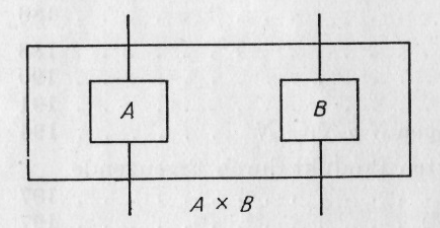
\includegraphics[]{figure1.png}
\label{fig:figure1}
\caption{}
\end{figure}

If $Z(A) = Q(B)$ we get from $A$ and $B$ a circuit $B\circ A$ by switching the $i$-th output of $A$ to the $i$-th input of $B$.

A circuit of elements of $\mathcal{U}$ is a device, which is described inductively by the preceding explanations.

If $\phi(A)$ ($\phi(B)$) is the function of circuit $A$ ($B$), then $\phi(A)\times \phi(B)$ is the function of $A\times B$, and $\phi(B)\circ \phi(A)$ for $Q(B) = Z(A)$  is the function of $B\circ A$.

The costs for the building blocks in $\mathcal{U}$ shall be defined by the function $L : \mathcal{U} \rightarrow N \cup {0}$. We define:

\[
\begin{array}{lcr}
L(A\times B) & = & L(A) + L(B), \\
L(A\circ B) & = & L(A) + L(B).
\end{array}
\]

Hereby a price is assigned to each circuit.

Now, the task is the following: Given $f : S^n \rightarrow S^m$, find a circuit $A$ with $\phi(A) = f$ and
\[
L(A) = \min_{B \in \phi^{-1}(f)} \{ L(B) \}.
\]

If $f$ does not fully map to $S^n$, but only to $R \subset S^n$, then the optimum shall be searched on $\cup_{g|R=f} \phi^{-1}(g)$. 

The task is generalized in an obvious way, if $Q(f) = Z(F) = S^n$ and $f$, as it is often the case with finite automata, is determined just by a transformation of $S^n$, 

In order to solve this problem it appears advantageous to know relations, which allow to generate from an element $A \in \phi^{-1}(f)$ all the elements from the class $\phi^{-1}(f)$.

In the first two sections of this work a theory of interconnection of automata will be developed, as already sketched out in the description of the task:

First, the topological notion of a \emph{flat} network is introduced. The binary operators "$\circ$" and "$\times$" will be explained for these networks. One obtains an algebraic structure $\mathcal{R}$, which is a category with respect to "$\circ$" and a semi-group with respect to "$\times$". $\mathcal{R}$ turns out to be a generalisation of the D-category (category with direct products), which we want to call \emph{$X$-Kategorie}.

$\mathcal{R}$ reflects the interconnection of automata, but does not reflect the possibility of different building blocks with the same number of inputs and outputs. This will be accommodated by assigning symbols of the alphabet $\mathcal{U}$ to inner points of the network, respecting the functions $Q : \mathcal{U} \rightarrow N \cup {0}$ and $Z : \mathcal{U} \rightarrow N \cup {0}$. One arrives at an $X$-Kategorie $\mathcal{F}(\mathcal{U})$, which possesses $\mathcal{U}$ as a free generator. The elements of $\mathcal{F}(\mathcal{U})$ correspond to the set of circuits which may be yielded from $\mathcal{U}$. The mapping $\phi$, which assigns to each automaton its functions, becomes a functor $\phi:\mathcal{F}(\mathcal{U}) \rightarrow \mathcal{C}$, where $\mathcal{C}$ is the category of mappings of type $S^n \rightarrow S^m$. 

The introduction of the quotient category  $\mathcal{F}(\mathcal{U})/\mathcal{R}$ from $\mathcal{F}(\mathcal{U})$ to a relational system $\mathcal{R}$ forms the basis for the study of classes $\phi^{-1}(f)$. In section 3 $\phi^{-1}(f)$ will be studied for certain categories $\mathcal{F(U)}$ and distinguished functors $\phi$: We consider only generators $\mathcal{U}$ with $\{U, V, D\} \subset \subset \mathcal{U}$ and $Z(A) = 1$ for $A\in \mathcal{U} \setminus \{U, V, D\}$ and functors $\phi$, for which $\phi(U)$ is the mapping from $S$
to $S^{\circ}$, $\phi(V)$ the permutation of the components of $S^2$, and $\phi(D)$ the diagonalisation $S \rightarrow S^2$. Such functions are called \emph{normal}. A relational system $\mathcal{R}$ will be given with the following property: For each normal $\phi$ it holds that $\phi(F) = \phi(G)$ for $F, G \in \mathcal{F}(\mathcal{U})$, iff $F\equiv G(\mathcal{R})$. $\mathcal{F}(\mathcal{U})/\mathcal{R}$ is a $D$-category and $\mathcal{U} \setminus \{U, V, D\}$ a free generator of the
$D$-category.

Thus, the relational system allows to simplify the representations $F$ of a function $\phi(F)$, which are possible without the knowledge of the elements in $\mathcal{U} \setminus \{ U, V, D \}$. Figure \ref{fig:figure2} shows that there are proper simplifications in this system.

\begin{figure}
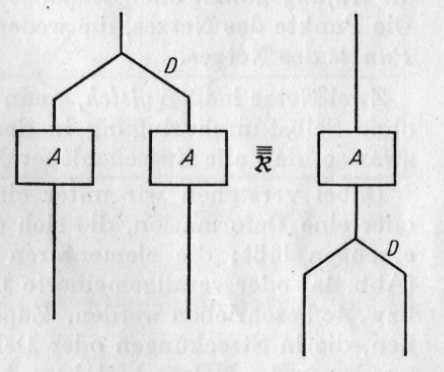
\includegraphics[]{figure2.png}
\label{fig:figure2}
\caption{}
\end{figure}

In this work we allow an arbitrary countable set for $S$, such that these results can also be of interest for computer programming. If one wants to formally simplify programs which are constructed from sub-programs, then the number of possible sub-programs renders the specific consideration of the computed function infeasible, but the rules for the transformation of programs have to be applicable uniformly for all sub-programs. Thus, that means that the allowed relations have to be the system
$\mathcal{R}$ or an equivalent system.

For an orientation on the state of the art of the theory of circuit synthesis refer to [2], in relation to Streckenkpomplexen to [5] and category theory to [4] and [6].
For stimulating discussions and critical remarks I want to thank J. D\"{o}rr and D. Puppe. My thanks go to the Deutsche Forschungsgemeinschaft, who has supported this study with a grant of the FRITZ-THYSSEN-foundation.

\end{document}
